\documentclass{beamer}
\setbeamertemplate{navigation symbols}{}

\usetheme{Madrid}
\usecolortheme{beaver}

% packages
\usepackage{graphicx}
\usepackage{enumitem}

% metadata
\title{Fault-Tolerant Quadcopter}
\author{Cooper, Vaughn, Mayank}
\date{\today}

\begin{document}

% title slide
{\setbeamertemplate{footline}{}
\begin{frame}
\begin{center}
{\Large\textbf{Fault-Tolerant Quadcopter}}\\
\vspace{\baselineskip}
ECE 453 Project Proposal (Fall 2018)\\
University of Wisconsin-Madison\\
\vspace{\baselineskip}
{\large\textit{Vaughn Kottler, Mayank Katwal, Cooper Green}}
\end{center}
\end{frame}
}

% state of the art (cheap toys)
\begin{frame}
\frametitle{State of the Art (Cheap Toys)}
\begin{center}
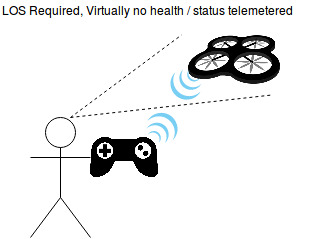
\includegraphics[width=3.5in]{../src/im/crude}

Price Range: \$25 - \$50
\end{center}
\end{frame}

% state of the art (fpv)
\begin{frame}
\frametitle{State of the Art (Enthusiast FPV)}
\begin{center}
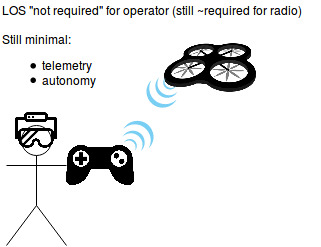
\includegraphics[width=3.5in]{../src/im/fpv}

Price Range: \$100+
\end{center}
\end{frame}

% state of the art (industry)
\begin{frame}
\frametitle{State of the Art (Industry)}
\begin{center}
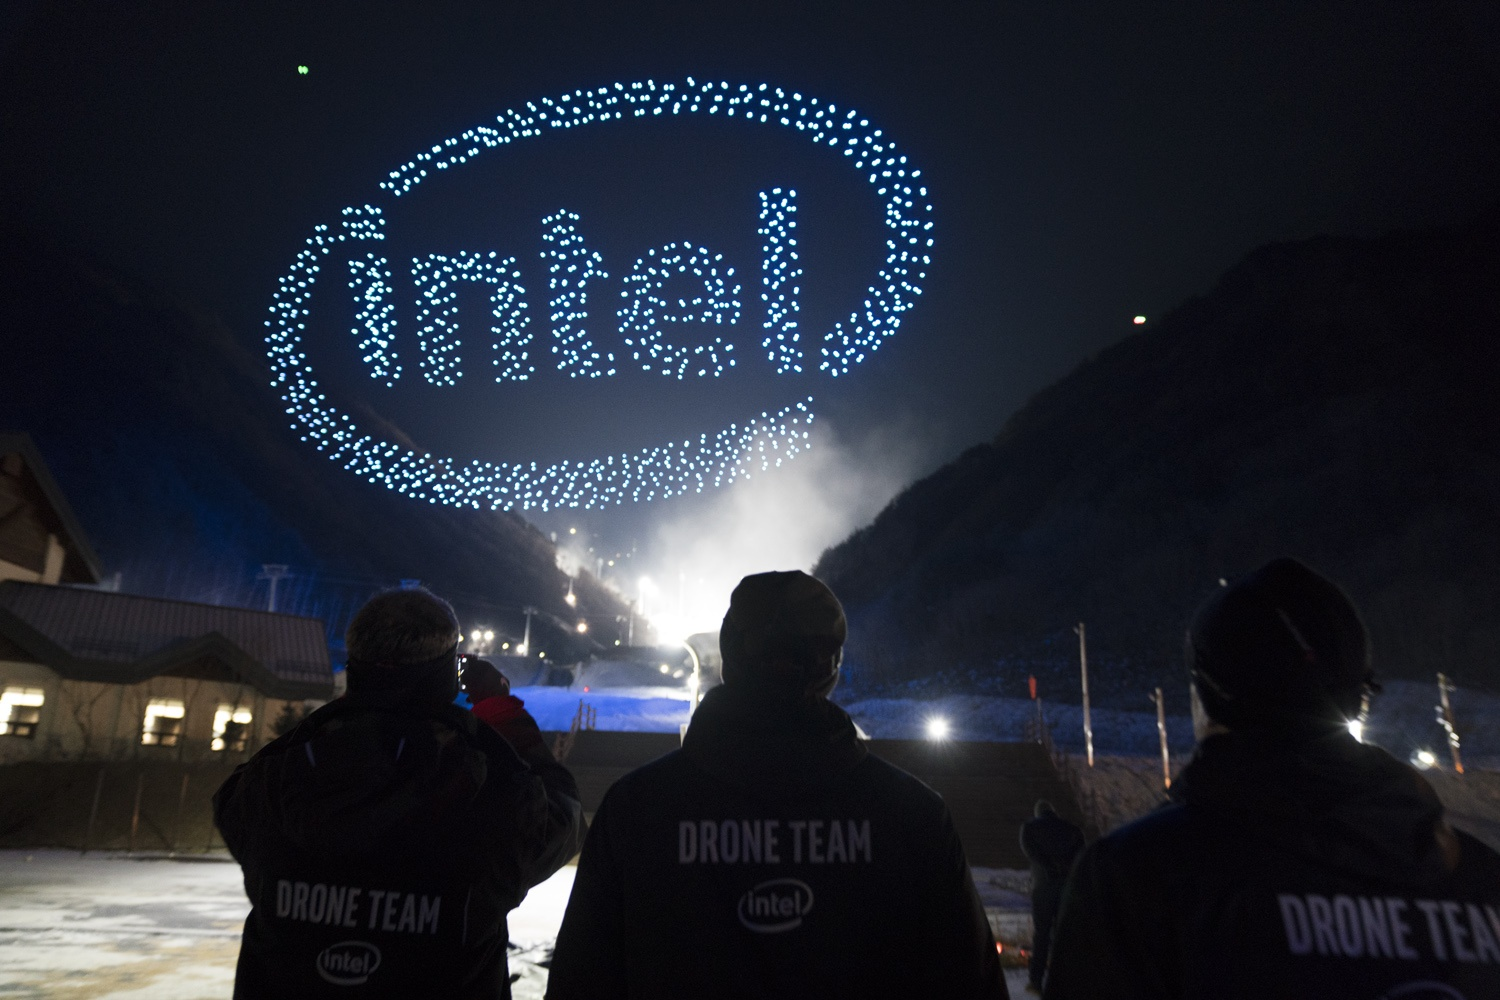
\includegraphics[width=4in]{../src/im/autonomous2}

Light Show at the Olympics
\end{center}
\end{frame}

% state of the art (industry)
\begin{frame}
\frametitle{State of the Art (Industry)}
\begin{center}
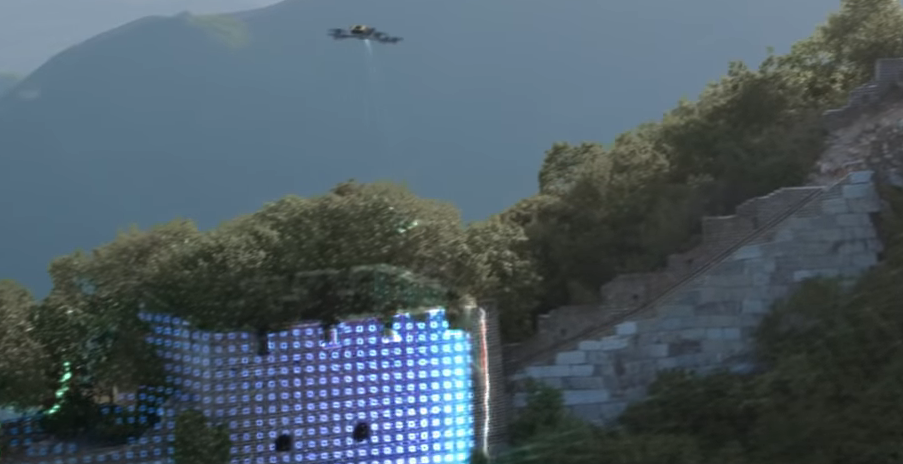
\includegraphics[width=4in]{../src/im/great_wall1}

Intel Surveys Great Wall of China
\end{center}
\end{frame}

% problem statement
\begin{frame}
\frametitle{Problem Statement}
\Large
No ``multi-vehicle fleet'' or autonomous-flight capable drone
technology available to interact with.
\break

\textbf{What gap can we fill in this ecosystem?}
\break

To gain experience with aerospace-related problems, we propose
designing, testing and building a custom flying machine.
\break

\textbf{How hard are these problems?}
\end{frame}

% concept of approach
\begin{frame}
\frametitle{Concept of Operation}
\begin{center}
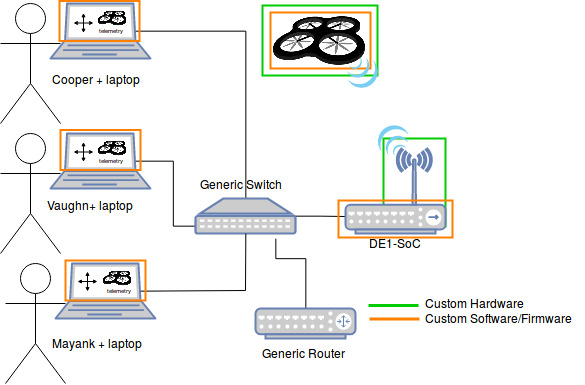
\includegraphics[width=4.5in]{../src/im/conops}
\end{center}
\end{frame}

% features
\begin{frame}
\frametitle{Features}
\begin{description}[align=right,labelwidth=130pt,itemsep=15pt]
    \item [Telemetry Viewing] -- View vehicle data from the UI
    \item [Manual Commanding] -- Control the vehicle from the UI
    \item [Holding-Pattern Stability] -- Ability to ``idle'' with little to no motion
	\item [Single-Fault Tolerant] -- Land safely if communication is lost
\end{description}
\end{frame}

% quadcopter
\begin{frame}
\frametitle{Quadcopter}
\begin{center}
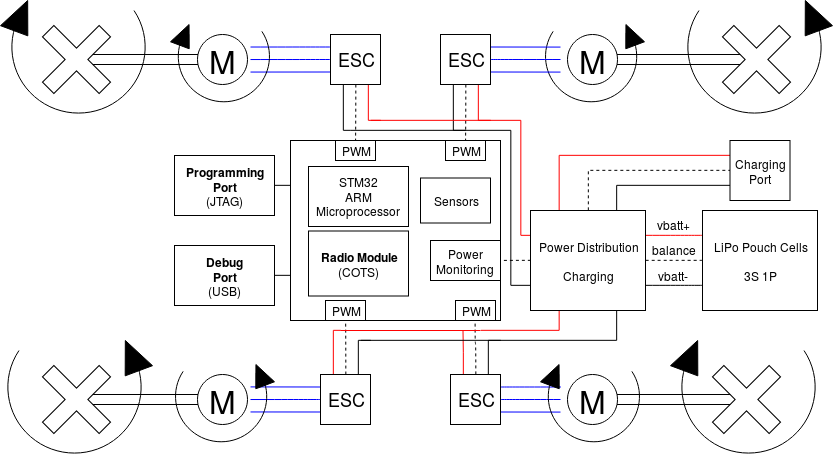
\includegraphics[width=\linewidth]{../src/im/quadcopter}
\end{center}
\end{frame}

% quadcopter components
\begin{frame}
\frametitle{Quadcopter Components}
\begin{center}
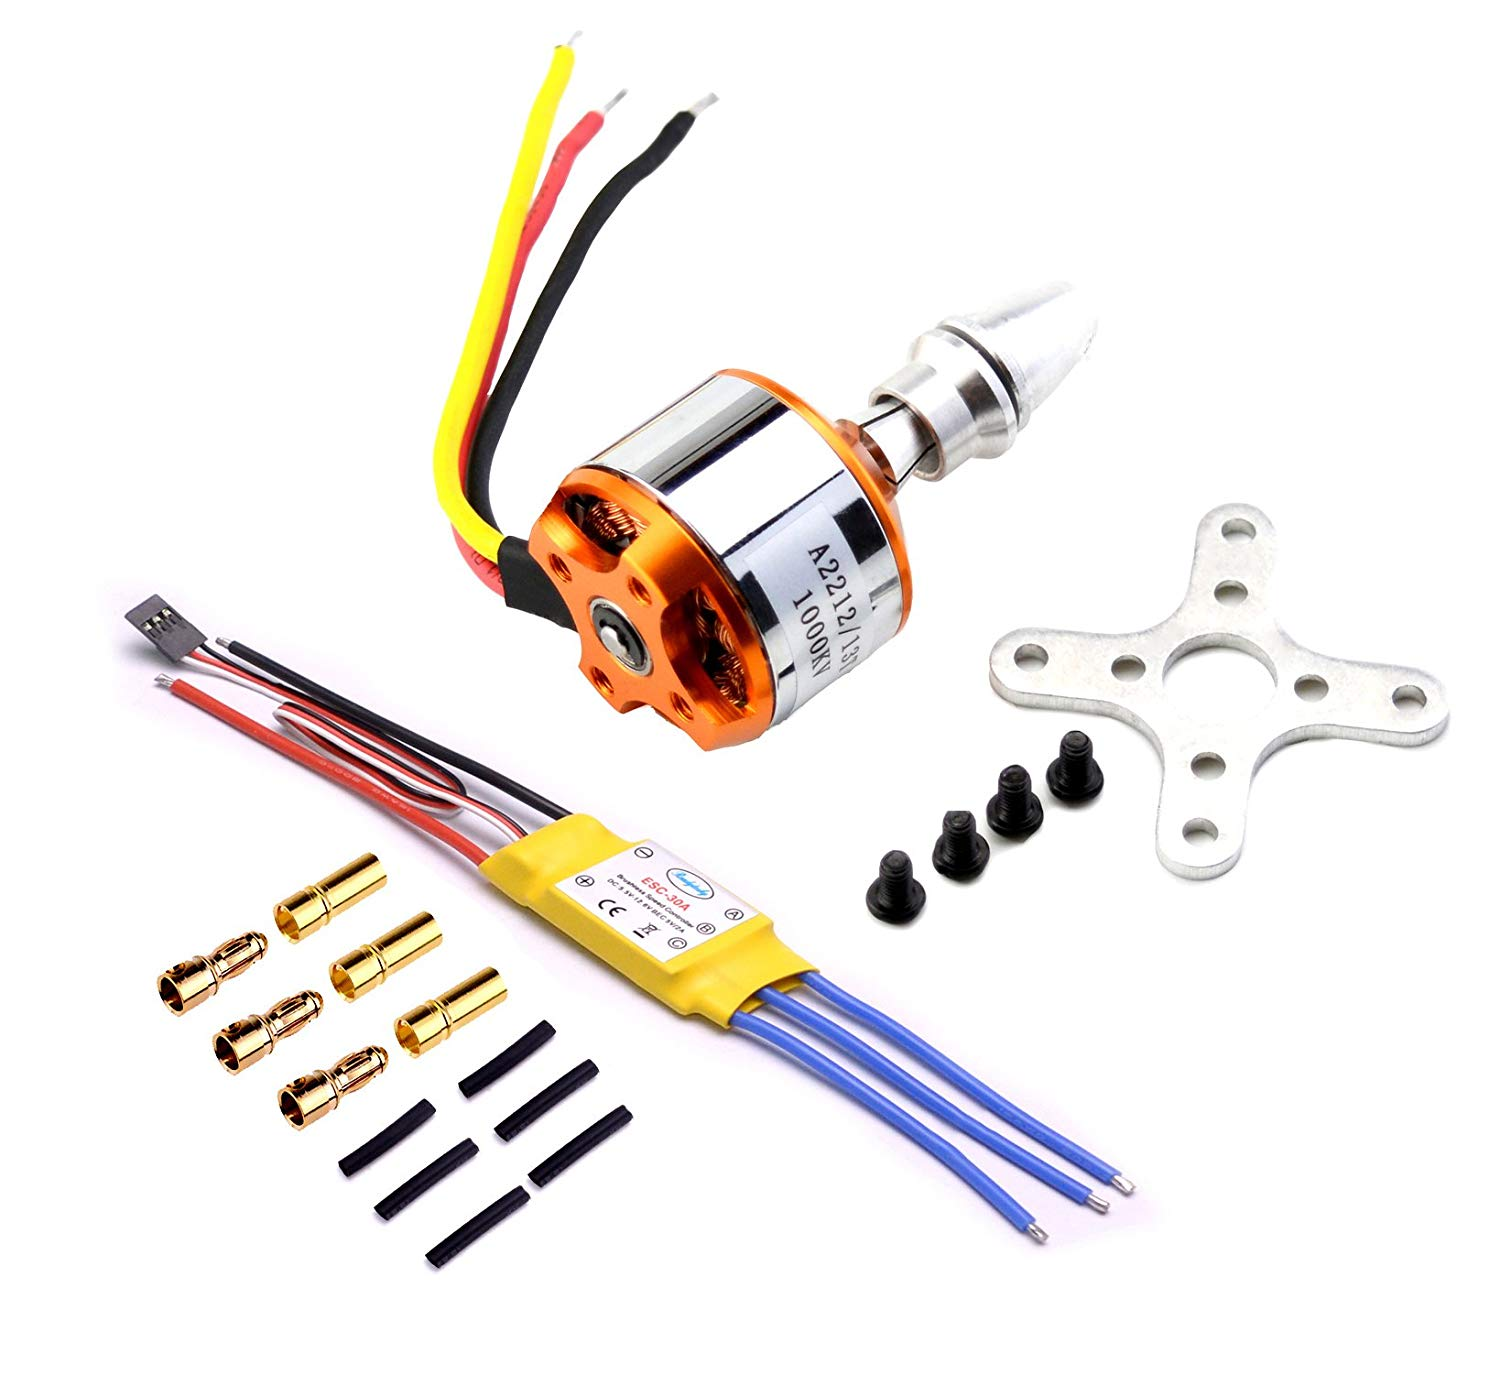
\includegraphics[width=1in]{../src/im/motor_esc}
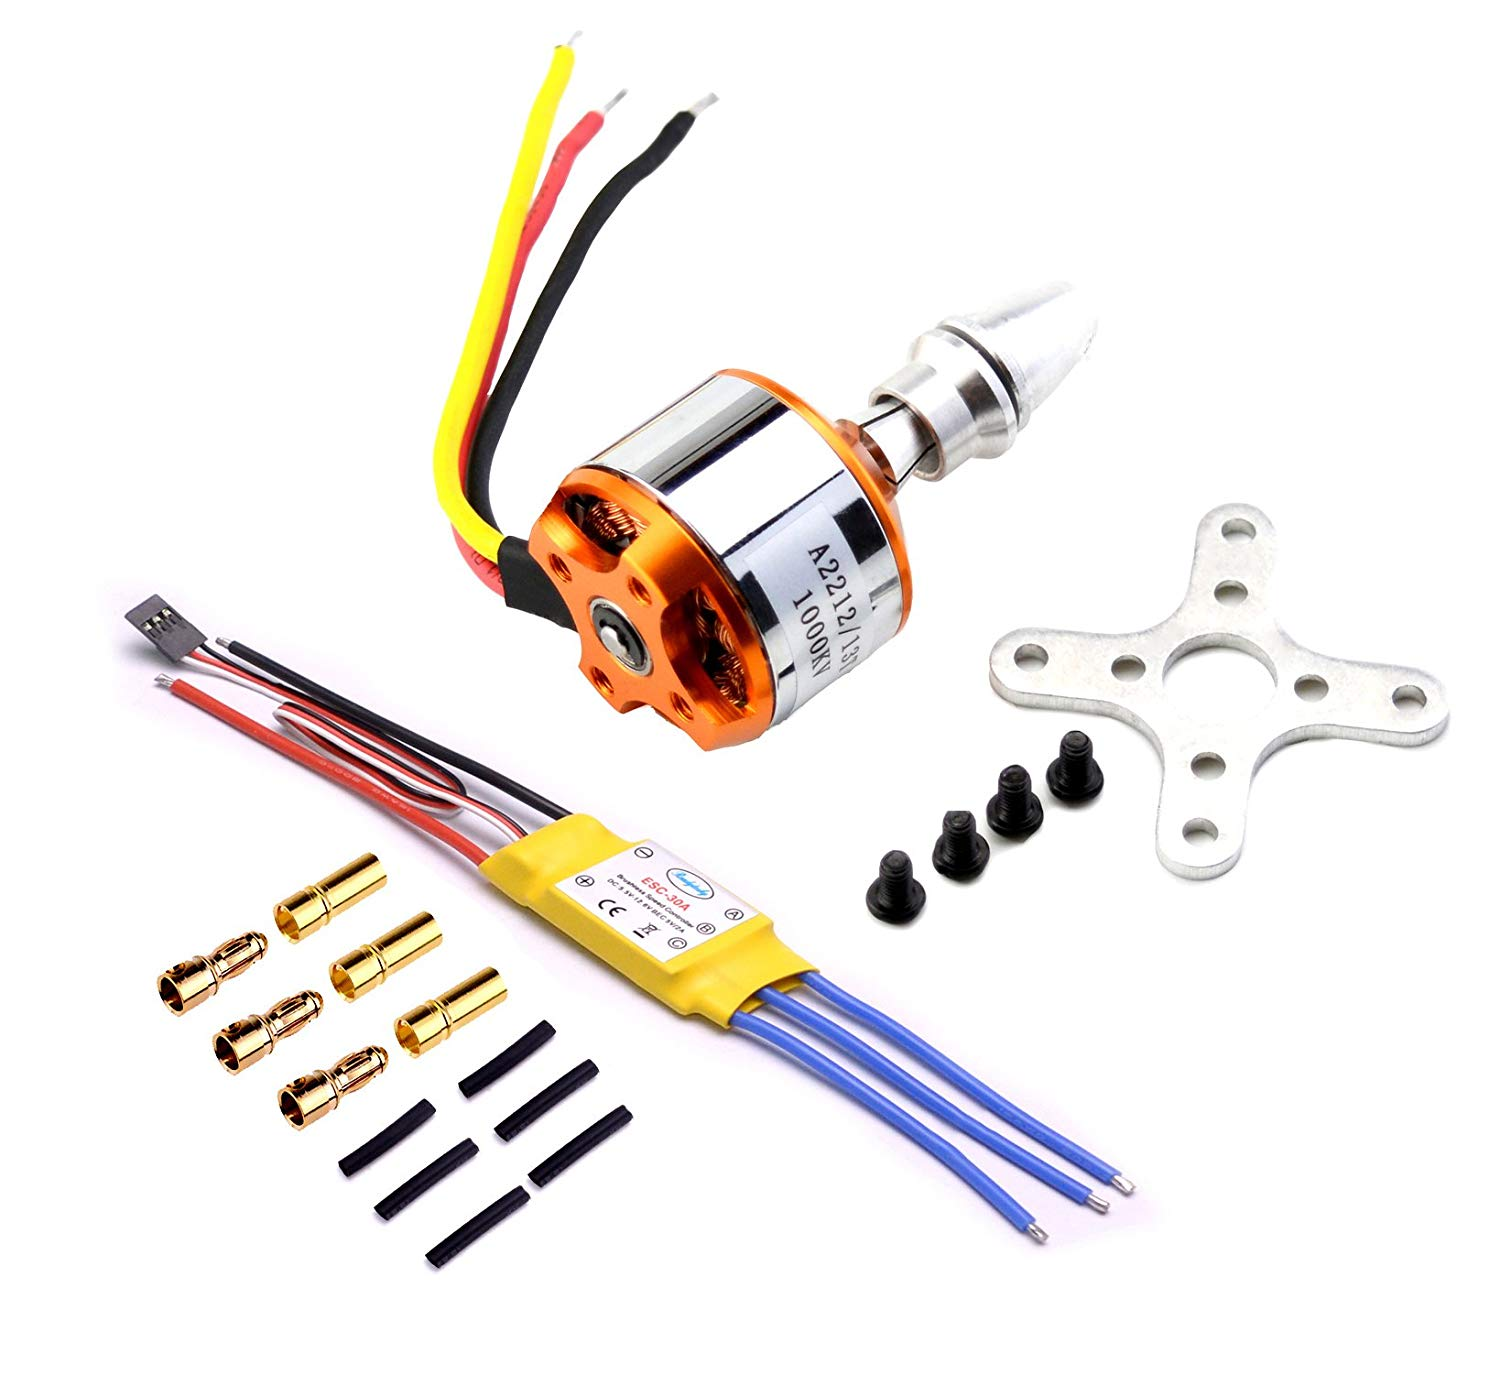
\includegraphics[width=1in]{../src/im/motor_esc}
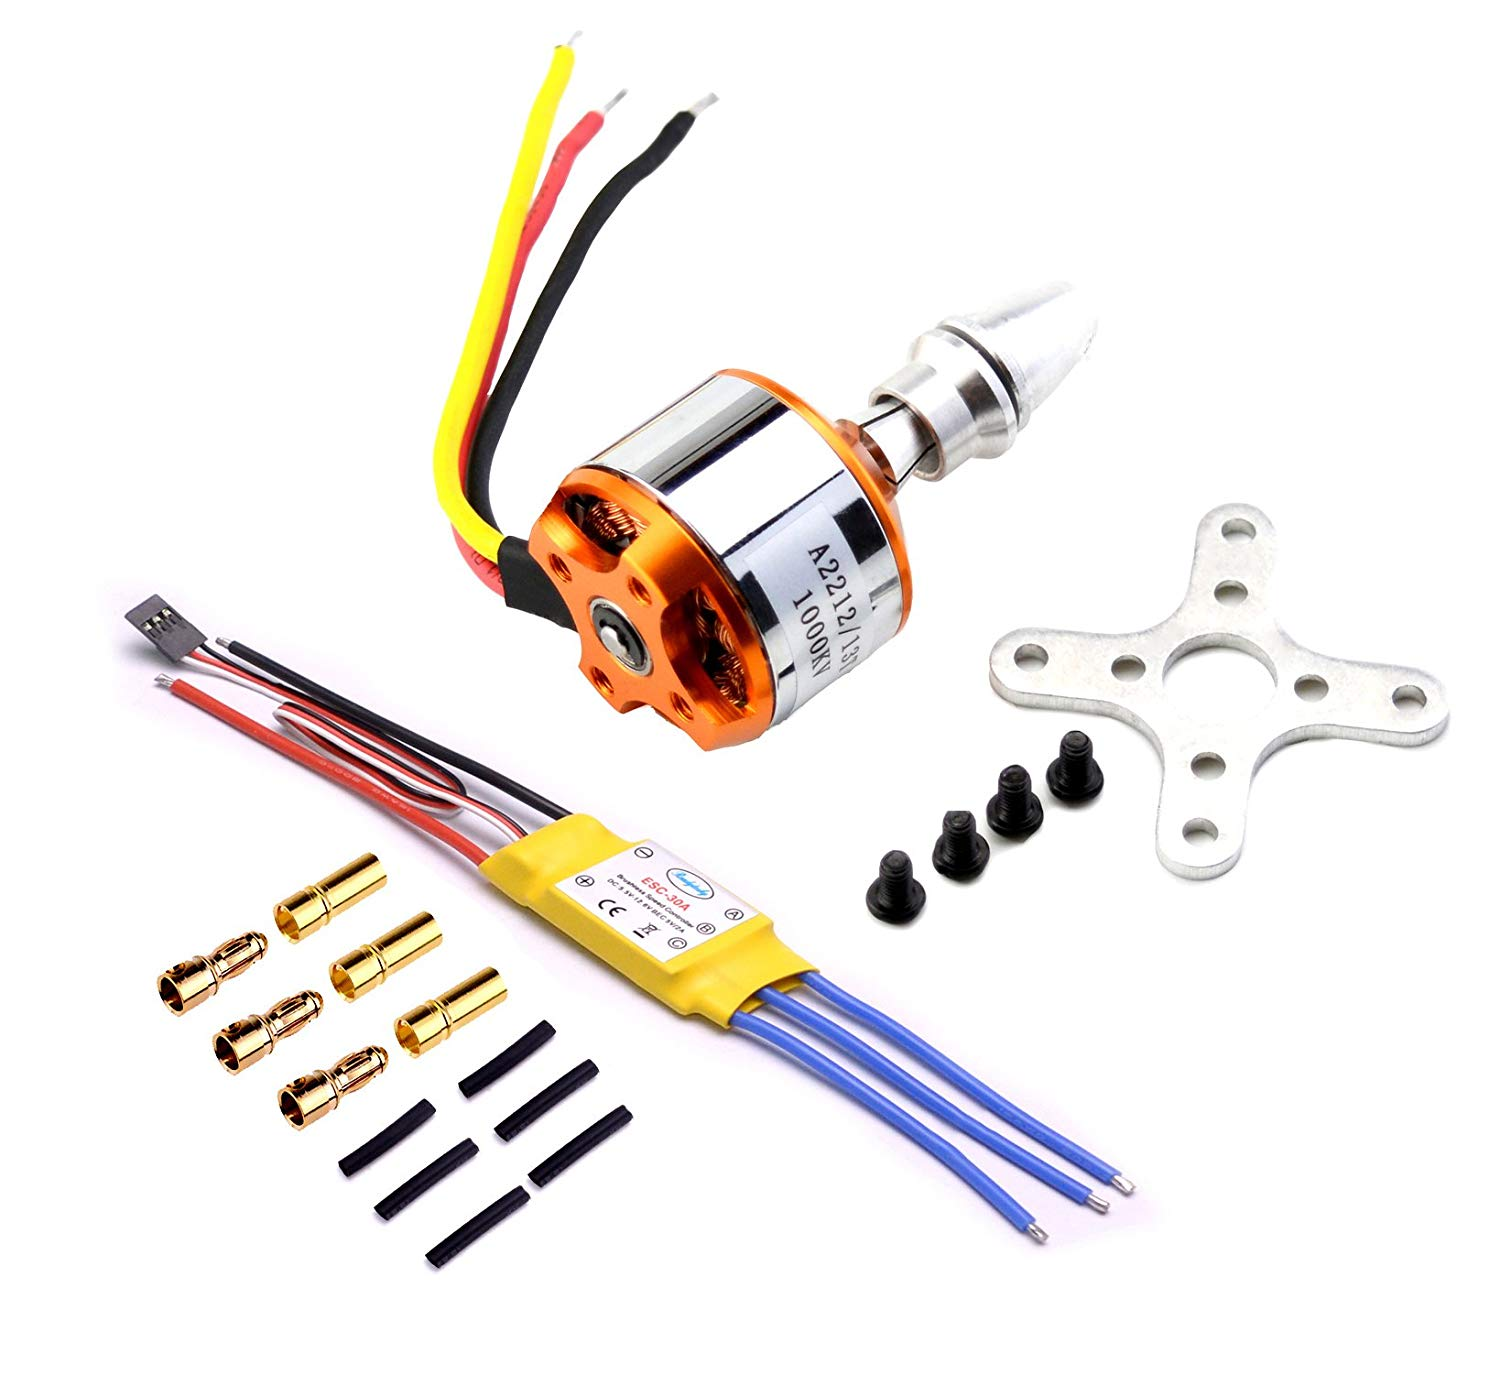
\includegraphics[width=1in]{../src/im/motor_esc}
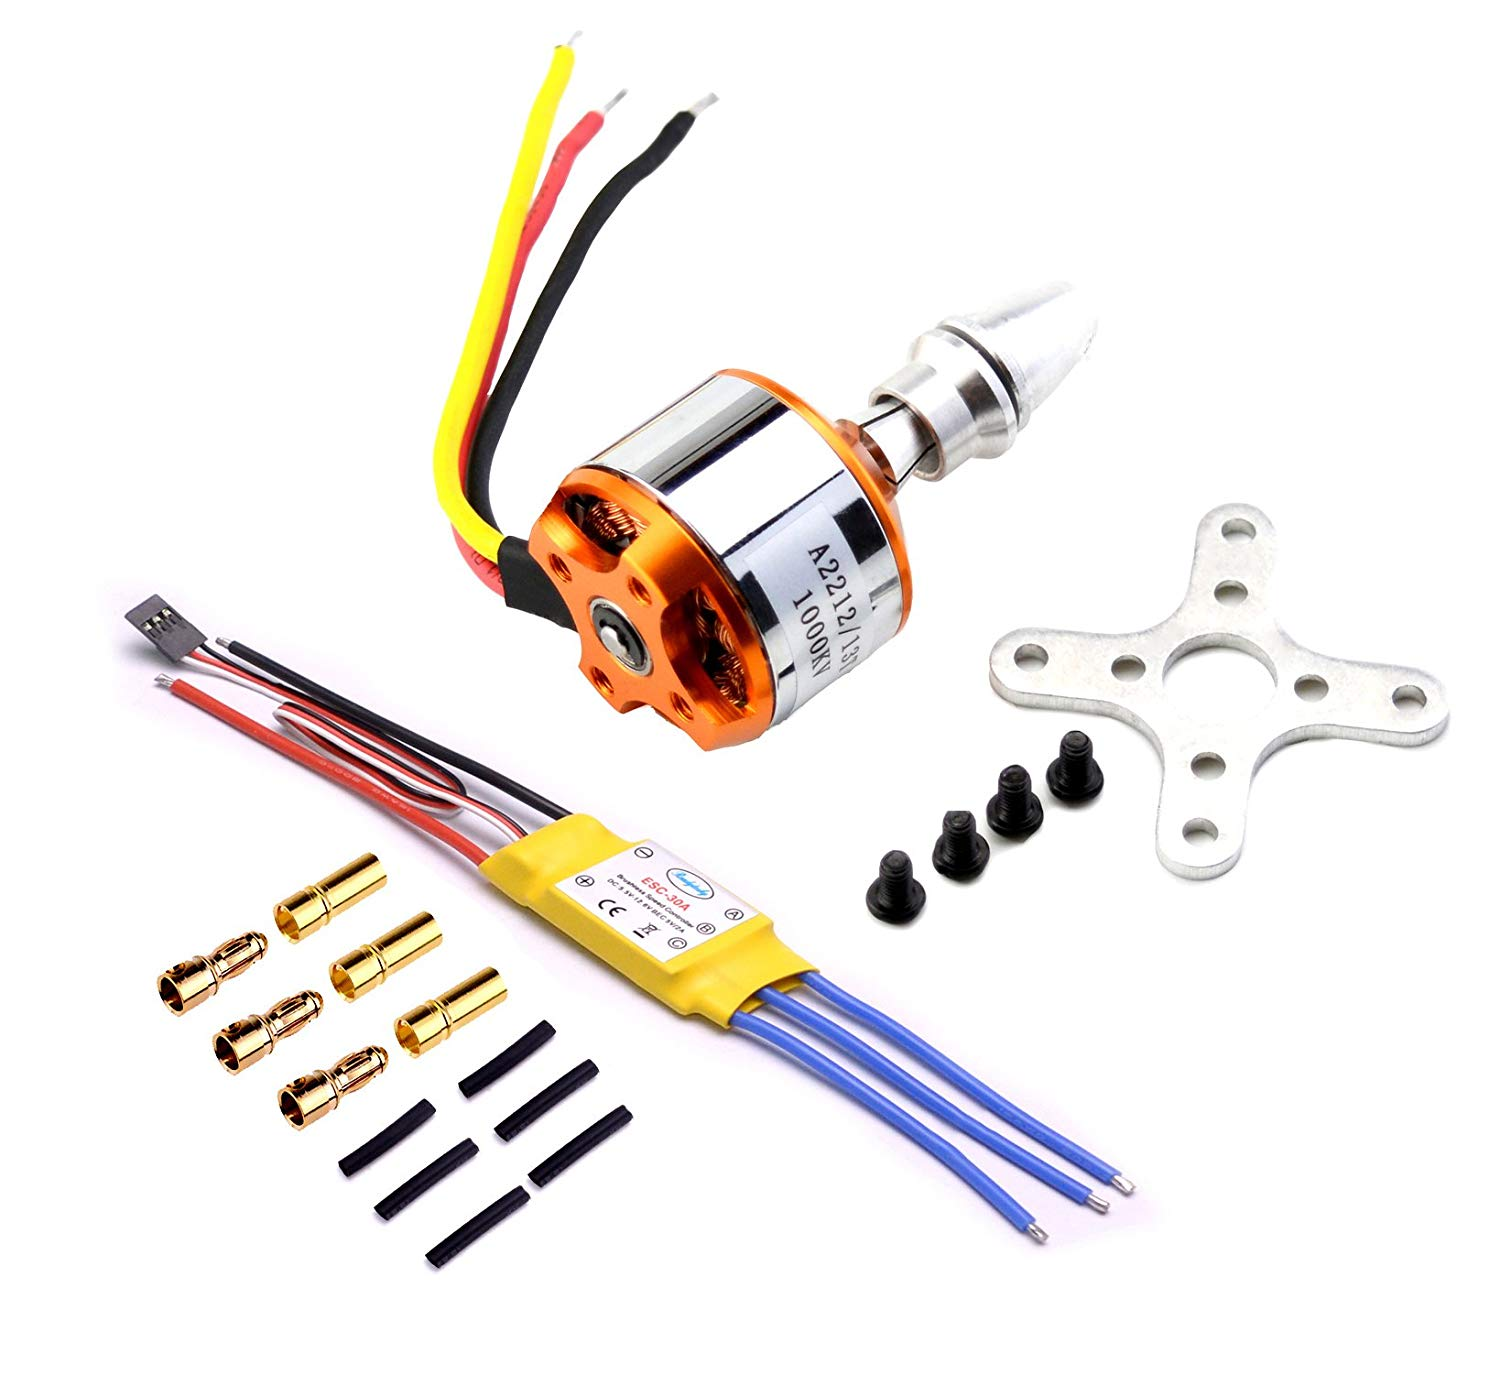
\includegraphics[width=1in]{../src/im/motor_esc}
\break
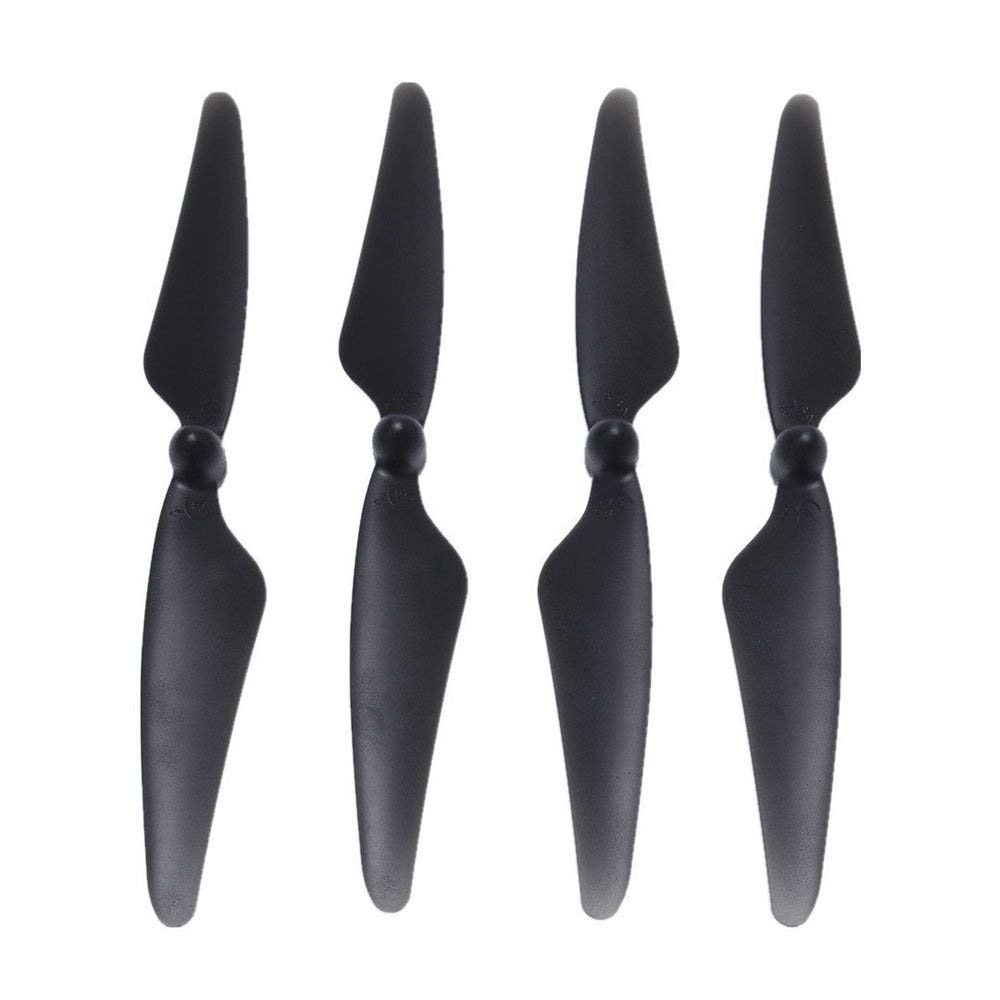
\includegraphics[width=1in]{../src/im/propeller}
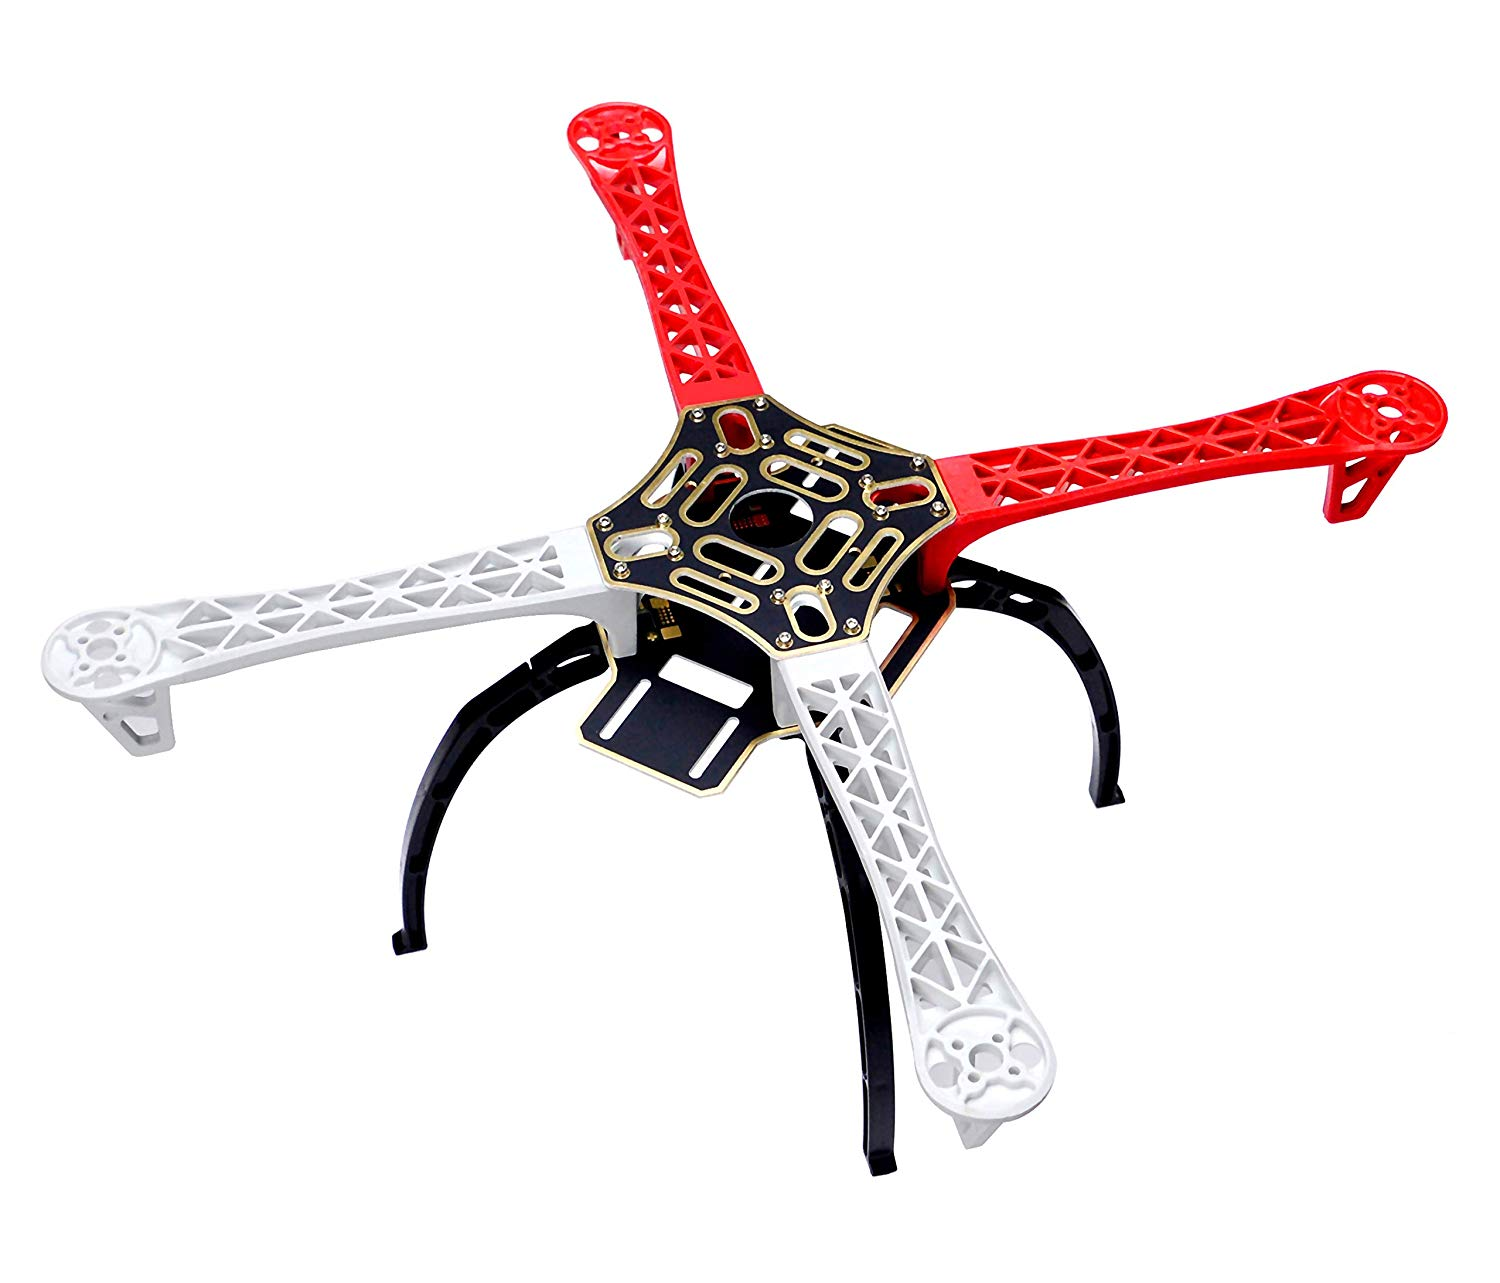
\includegraphics[width=1in]{../src/im/chassis}
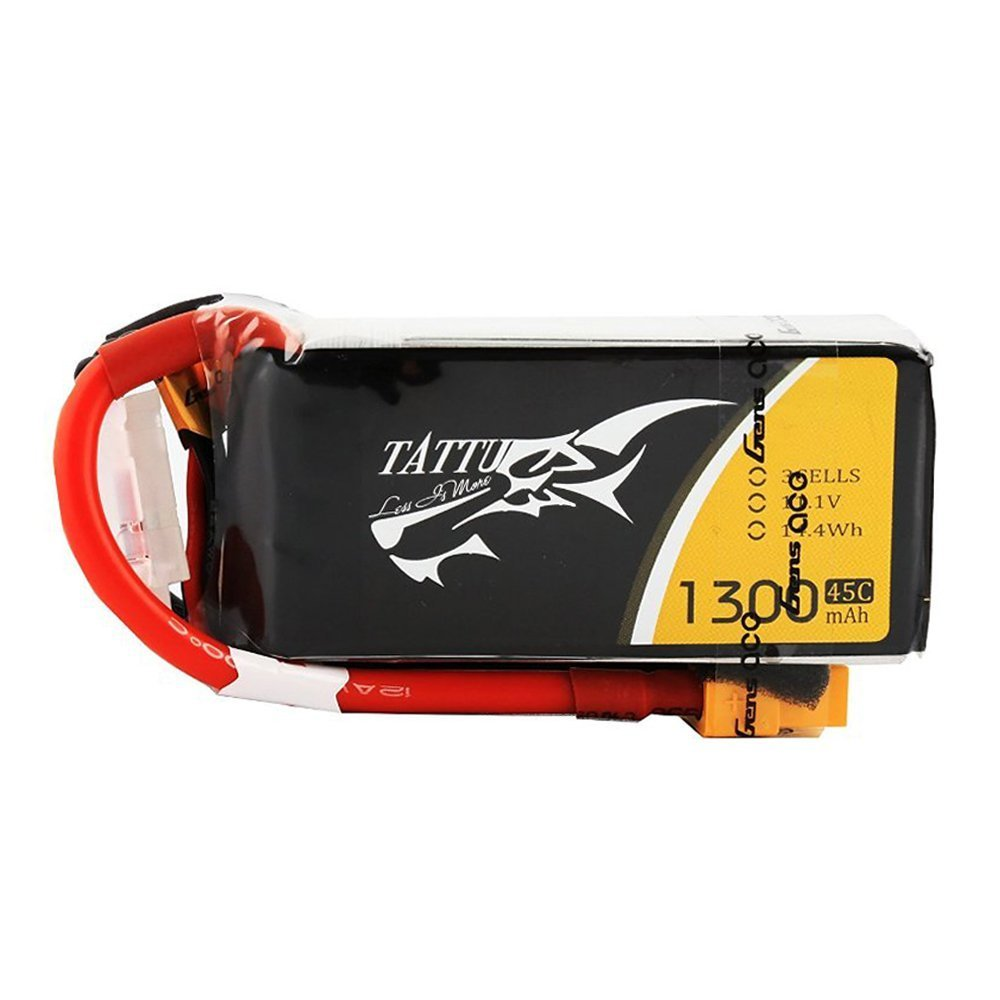
\includegraphics[width=1in]{../src/im/battery}
\break
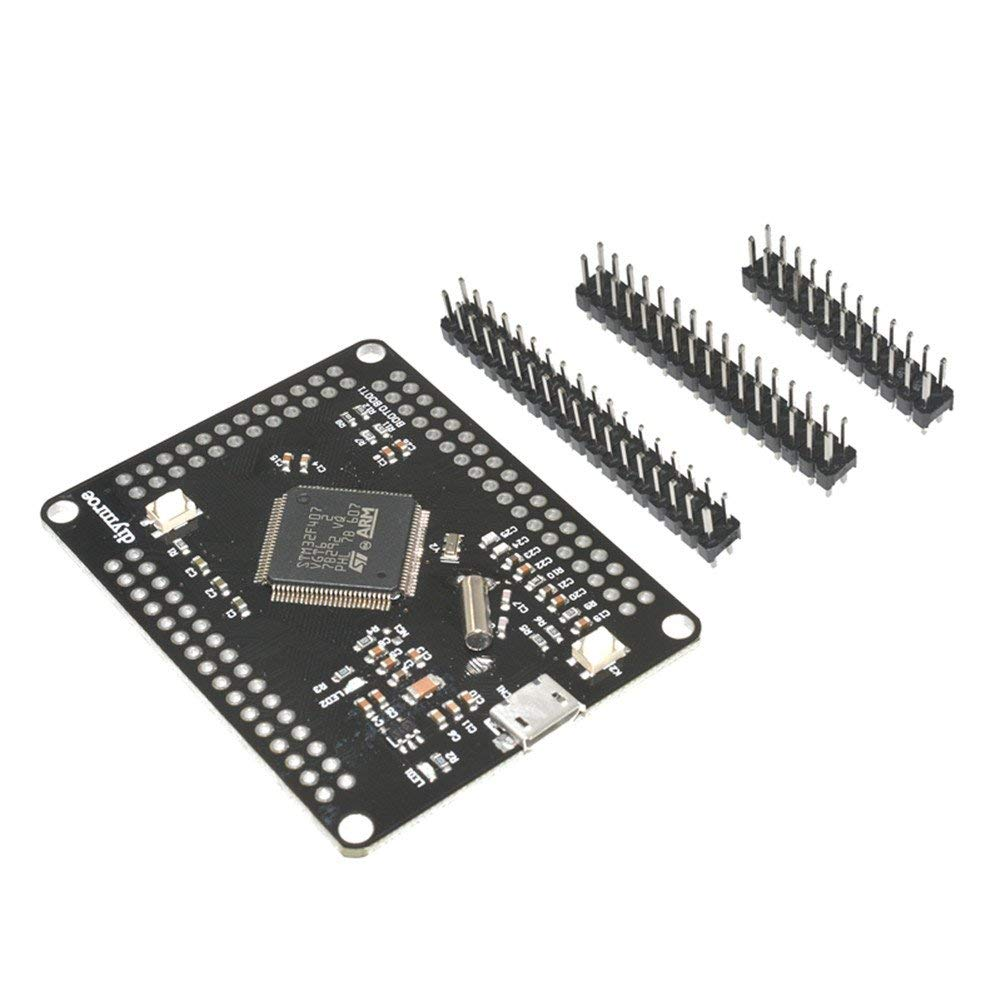
\includegraphics[width=1in]{../src/im/dev_board}
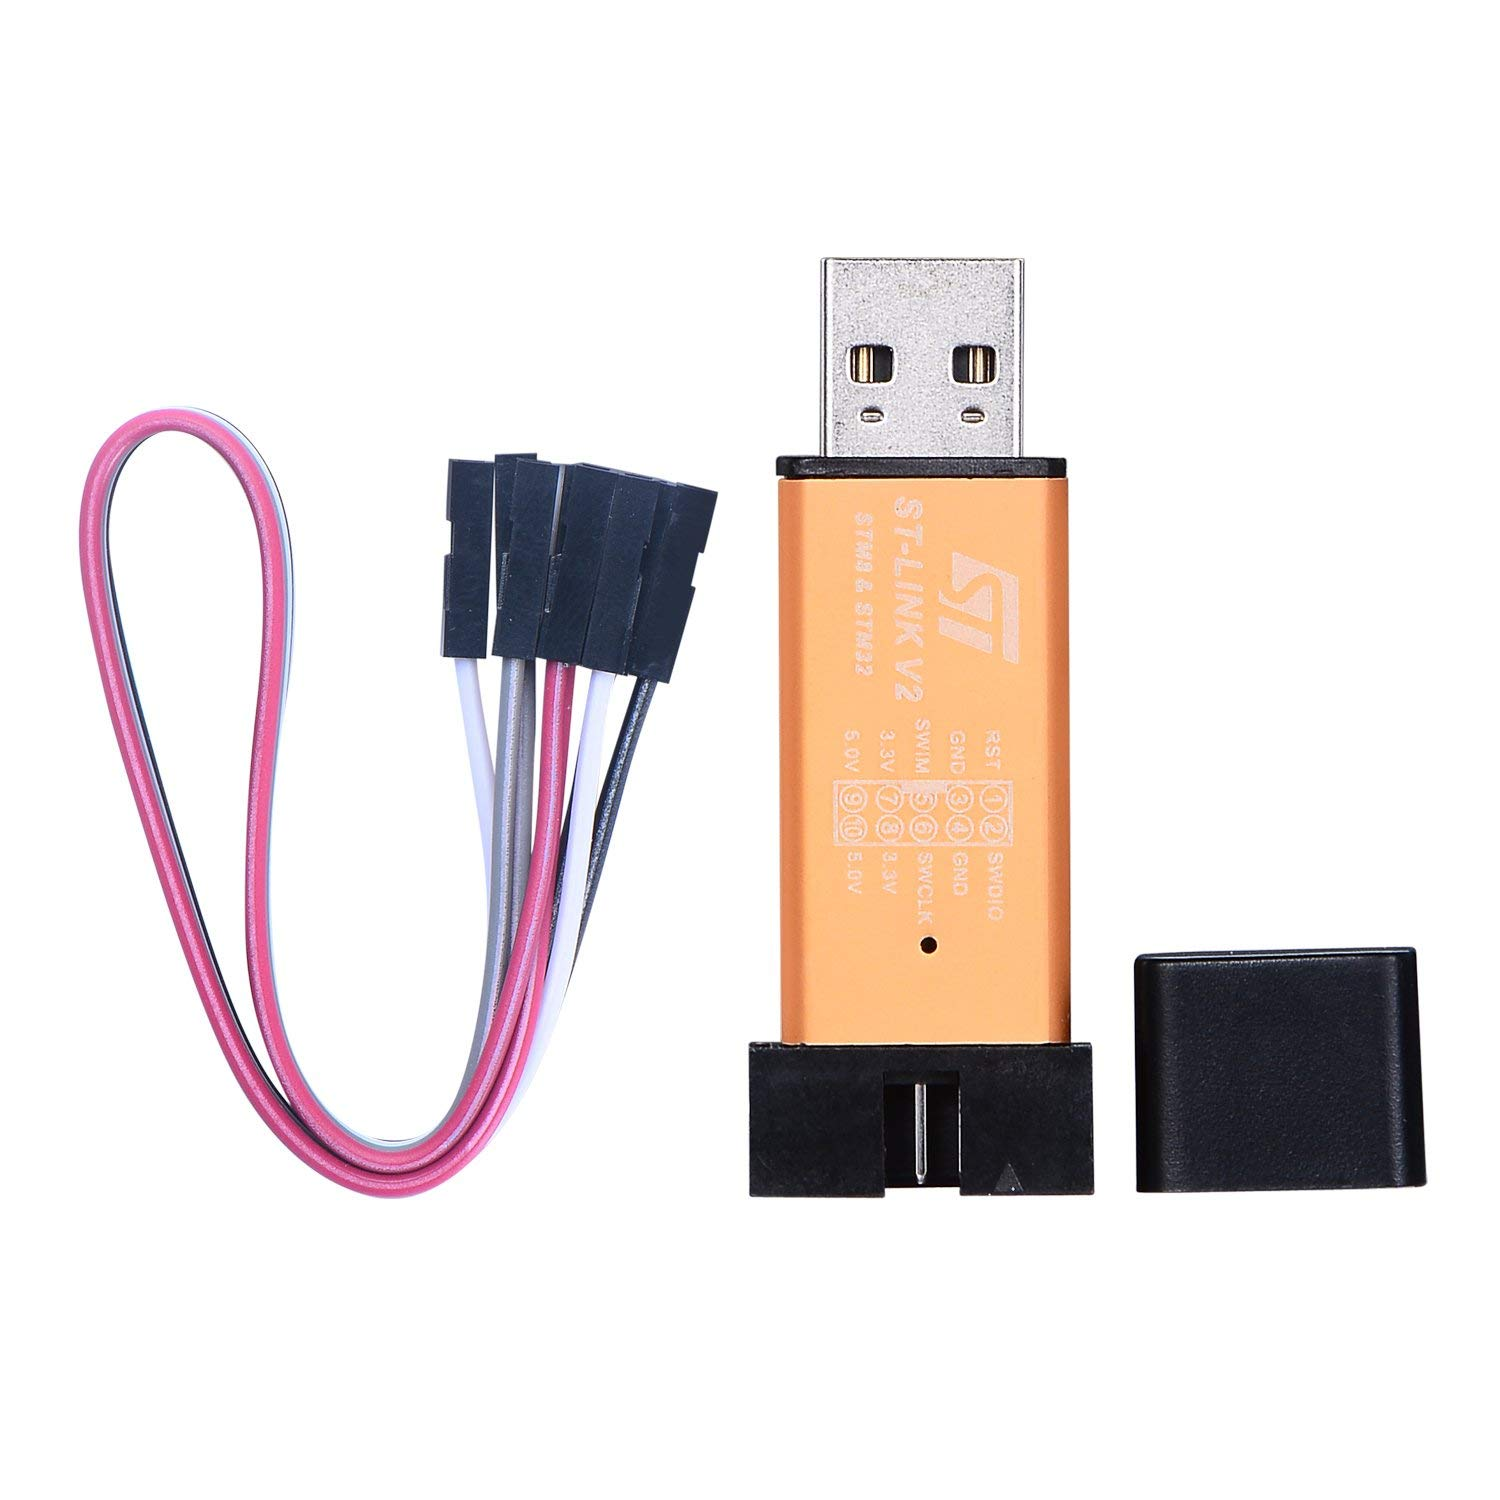
\includegraphics[width=1in]{../src/im/programmer}
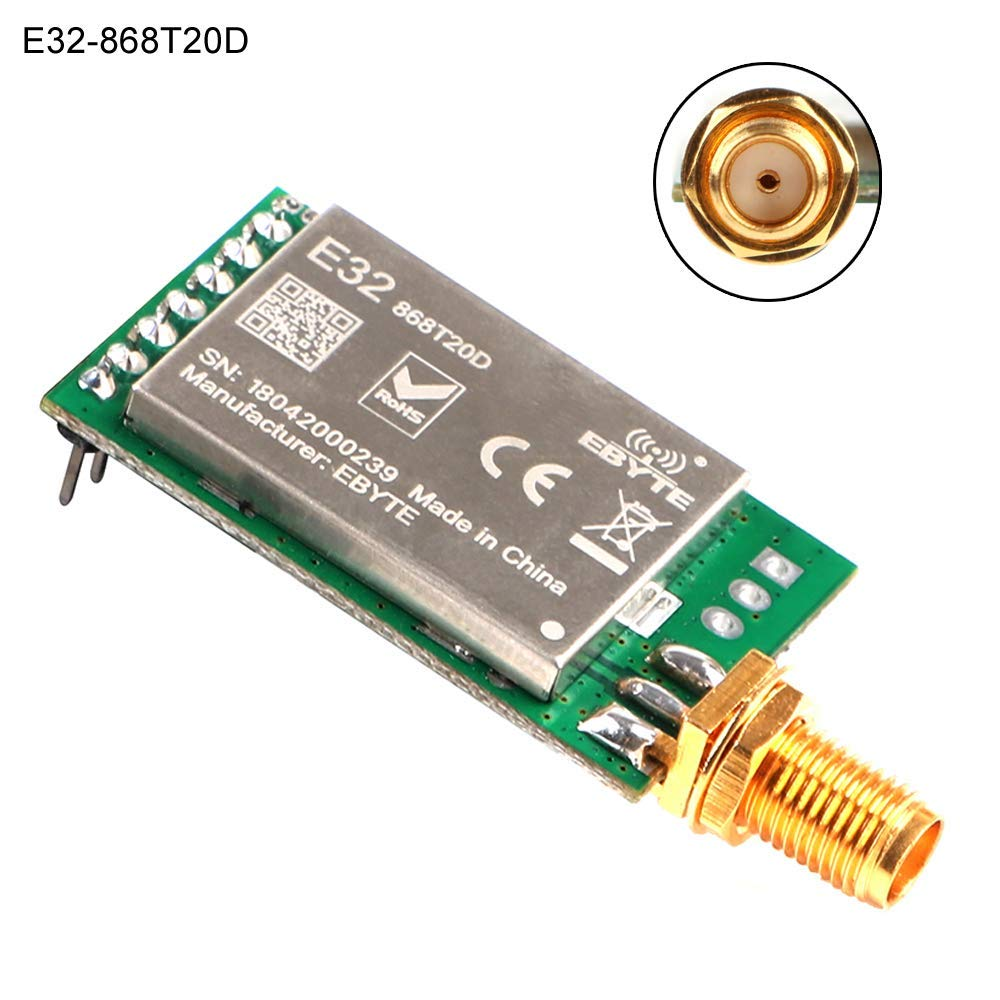
\includegraphics[width=1in]{../src/im/radio1}
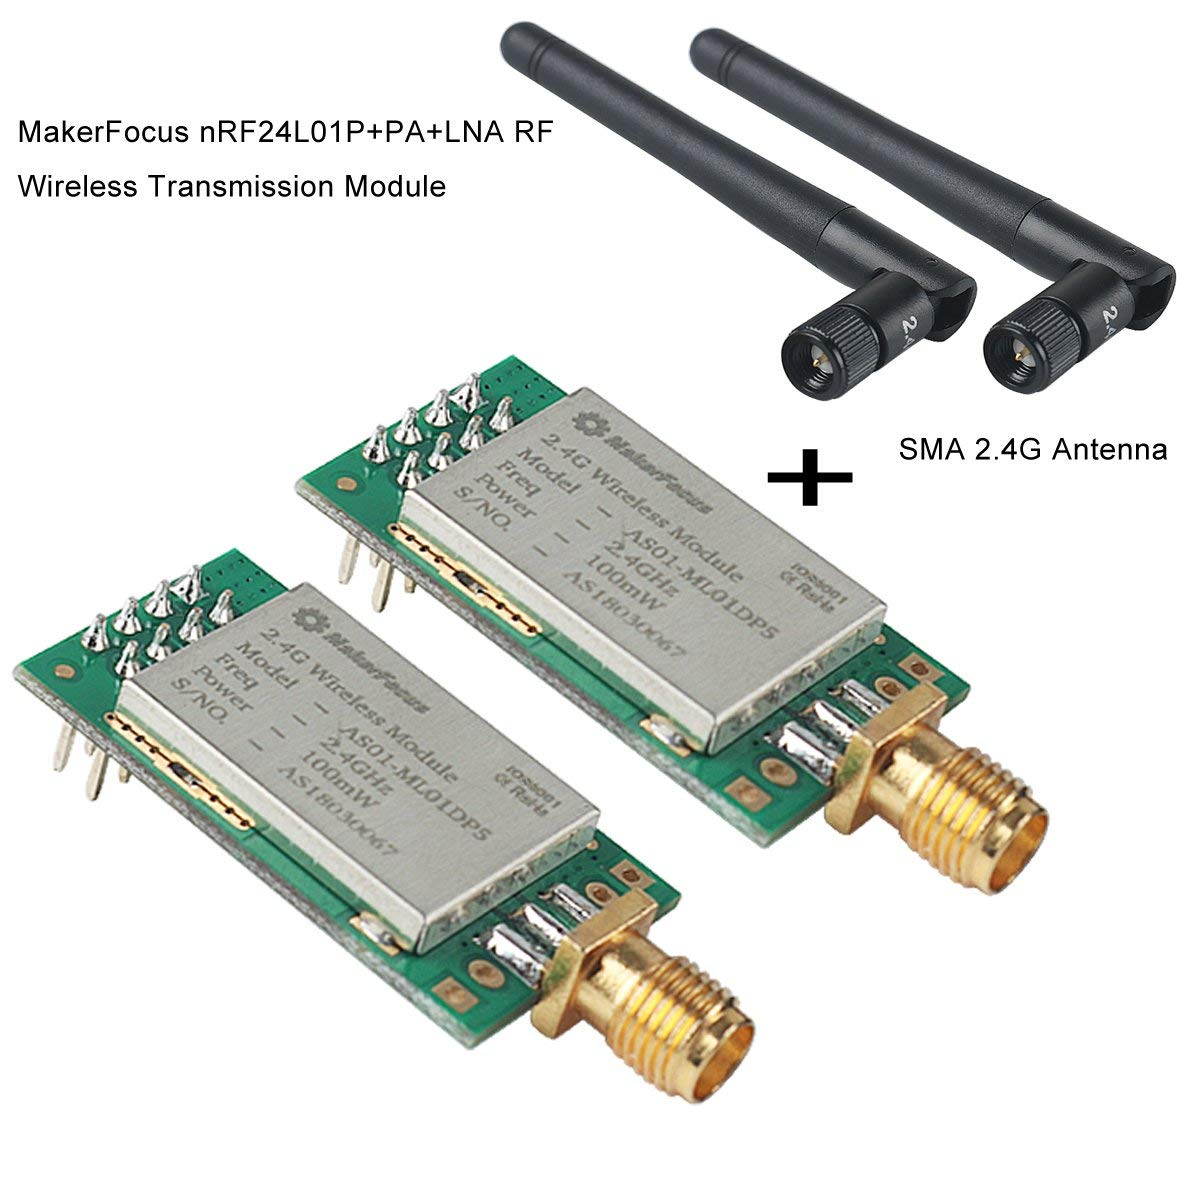
\includegraphics[width=1in]{../src/im/radio2}
\end{center}
\end{frame}

% ground station
\begin{frame}
\frametitle{Ground Station}
\begin{center}
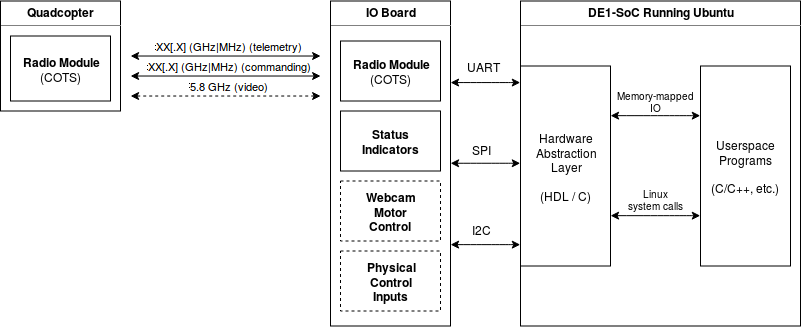
\includegraphics[width=\linewidth]{../src/im/ground_station}
\end{center}
\end{frame}

% display and controller
\begin{frame}
\frametitle{User Interface}
\begin{center}
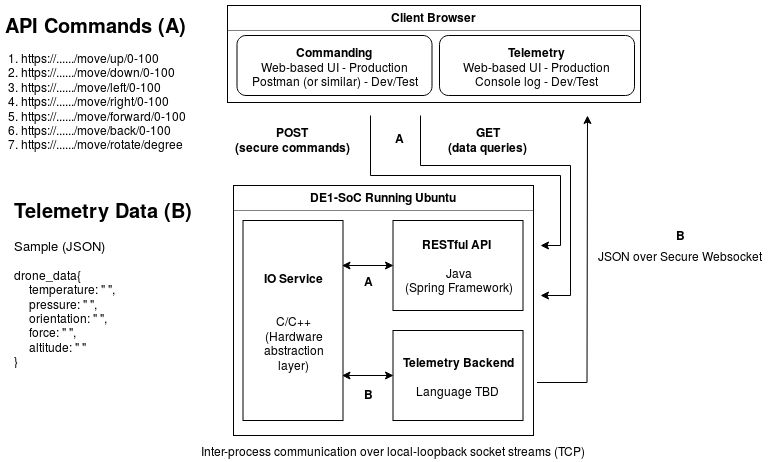
\includegraphics[height=225pt,width=\linewidth,keepaspectratio]{../src/im/display_controller}
\end{center}
\end{frame}

% total cost
\begin{frame}
\frametitle{Estimated Total Cost}
\large
\vspace{0.2in}
\begin{itemize}
\item \textbf{\$305} -- Quadcopter (Parts, custom PCB)
\item \textbf{\$108} -- Ground Station (Parts, custom PCB)
\item \textbf{\$200} -- General development and test equipment/components
\item \textbf{\$613} -- Total
\end{itemize}
\vspace{0.2in}
\Large
Higher-granularity breakdown in report.
    
\end{frame}

\begin{frame}
\frametitle{Summary}
\large
We feel prepared to take on this challenge:
\begin{itemize}
    \item[\textbullet] Prior experience with systems' engineering (vehicle projects)
    \item[\textbullet] At least a dozen previous failures
    \item[\textbullet] Confident in this architecture
    \item[\textbullet] Have development tools and equipment on standby
\end{itemize}
\vspace{0.5in}
\begin{center}
Funding would greatly increase the quality of the final product!
\end{center}
\end{frame}

\end{document}
